%%%%%%
%
% $Author: Abishek $
% $Date: 06.05.2024 $
% $Path: BA24-02-Time-Series\report\Contents\en$
% $Version: 1.0 $
%
%
% !TeX encoding = utf8
% !TeX root = Rename
% !TeX TXS-program:bibliography = txs:///bibtex

\chapter{Development Environment}
\section{Python}

Python is a popular programming language known for its simplicity and readability, making it ideal for beginners. It is widely used in tasks like data analysis, machine learning, and visualization, which are essential for recognizing gait patterns. Python's extensive library ecosystem helps you perform complex tasks like data cleaning, creating graphs, and building prediction models with minimal effort\cite{Python:2024}.

\subsection{Version}
Use Python 3.9 or newer. Older versions might not support some libraries used for machine learning and data processing.\cite{PythonGuide:2023}

\subsection*{Installation}
Python installation varies across operating systems. Follow the steps below for your platform to set up Python successfully:

\begin{itemize}
	\item \textbf{Windows:}
	\begin{enumerate}
		\item Visit the official Python downloads page:
		 \item\href{https://www.python.org/downloads}{https://www.python.org/downloads}.
		\item Download the installer for Windows.
		\item Run the installer and ensure the checkbox for \textbf{"Add Python to PATH"} is selected. This ensures you can run Python from any command prompt without additional setup.
		\item Click "Install Now" and wait for the process to complete.
		\item To verify the installation, open the Command Prompt (\texttt{cmd}) and type:
		\begin{lstlisting}[language=bash]
			python --version
		\end{lstlisting}
		If Python is installed correctly, this will display the installed version number.
	\end{enumerate}
	
	
	\item \textbf{Linux:}
	\begin{enumerate}
		\item For most Linux distributions, Python is pre-installed. However, you may need to update it or install additional tools like \texttt{pip} (Python’s package manager).
		\item Update the system's package list:
		\begin{lstlisting}[language=bash]
			sudo apt update
		\end{lstlisting}
		\item Install Python and \texttt{pip}:
		\begin{lstlisting}[language=bash]
			sudo apt install python3 python3-pip
		\end{lstlisting}
		\item Verify installation:
		\begin{lstlisting}[language=bash]
			python3 --version
			pip3 --version
		\end{lstlisting}
	\end{enumerate}
	
	\item \textbf{macOS:}
	\begin{enumerate}
		\item Python can be installed on macOS using \texttt{Homebrew}, a popular package manager for macOS.
		\item Open the Terminal and install Homebrew if it’s not already installed:
		\begin{lstlisting}[language=bash]
			/bin/bash -c "$(curl -fsSL https://raw.githubusercontent.com/Homebrew/install/HEAD/install.sh)"
		\end{lstlisting}
		\item Use Homebrew to install Python:
		\begin{lstlisting}[language=bash]
			brew install python
		\end{lstlisting}
		\item Verify installation:
		\begin{lstlisting}[language=bash]
			python3 --version
			pip3 --version
		\end{lstlisting}
	\end{enumerate}
\end{itemize}
	
	
	These steps ensure that Python is installed and configured correctly for use in projects like gait pattern recognition.
	
	
	\subsection*{Configuration}
	\begin{enumerate}
		\item Create a virtual environment to manage dependencies:
		\begin{lstlisting}[language=bash]
			python -m venv gait_env
		\end{lstlisting}
		\item Activate the virtual environment:
		\begin{itemize}
			\item On Windows:
			\begin{lstlisting}[language=bash]
				gait_env\Scripts\activate
			\end{lstlisting}
			\item On Linux/macOS:
			\begin{lstlisting}[language=bash]
				source gait_env/bin/activate
			\end{lstlisting}
		\end{itemize}
		\item Install required libraries:
		\begin{lstlisting}[language=bash]
			pip install numpy pandas matplotlib scikit-learn tensorflow
		\end{lstlisting}
	\end{enumerate}
	\begin{itemize}
		\item \textbf{NumPy:} For efficient mathematical operations on multi-dimensional arrays from sensor readings\cite{NumPy:2024}.
		\item \textbf{Pandas:} For organizing IMU data into a structured, tabular format and performing statistical summaries\cite{Pandas:2024}.
		\item \textbf{Matplotlib:} To plot sensor readings, compare gait cycles, and visualize classification results\cite{Matplotlib:2024}.
		\item \textbf{Scikit-learn:} For training lightweight models, feature extraction, and evaluating performance metrics\cite{Scikit-Learn:2024}.
		\item \textbf{TensorFlow:} For deep learning-based approaches when large datasets are available or complex features need to be automatically learned\cite{TensorFlow:2024}.
	\end{itemize}
	\subsection*{First Steps}
	Before you start writing your Python code, it is essential to choose an environment where you will write and execute your scripts. Using an IDE (Integrated Development Environment) or a text editor is recommended because they provide features such as syntax highlighting, debugging tools, and code suggestions, which simplify programming and reduce errors.\cite{PythonGuide:2023}
	
	\begin{enumerate}
		\item \textbf{Open a Python IDE or a text editor:} \\
		Examples include Visual Studio Code (VS Code), PyCharm, or a basic text editor like Notepad++.
		\begin{itemize}
			\item IDEs like VS Code or PyCharm offer features like auto-completion, integrated terminal, and debugging tools, making them ideal for larger projects\cite{Pycharm:2024}.
			\item Text editors like Notepad++ or Sublime Text are lightweight and suitable for smaller scripts or quick edits.
		\end{itemize}
		
		\item \textbf{Create a Python file:} \\
		Create a new file in your IDE or text editor and save it with a \texttt{.py} extension (e.g., \texttt{hello.py}). The \texttt{.py} extension indicates that the file contains Python code and allows it to be executed by the Python interpreter.
	\end{enumerate}
	
		\subsection*{Program ``Hello World''}
	\begin{lstlisting}[language=Python, caption=Python Hello World Program]
		# Hello World Program
		print("Hello, World!")
	\end{lstlisting}
	To run:
	\begin{enumerate}
		\item Save the file as \texttt{hello.py}.
		\item Open a terminal, navigate to the file's location, and run:
		\begin{lstlisting}[language=bash]
			python hello.py
		\end{lstlisting}
		\item Output:
		\begin{lstlisting}
			Hello, World!
		\end{lstlisting}
	\end{enumerate}
	
\section{Arduino IDE}

The Arduino Integrated Development Environment (IDE) is a versatile and user-friendly platform designed for writing, compiling, and uploading code to Arduino-compatible boards, such as the Arduino Nano 33 BLE Sense. It supports a wide range of libraries and hardware, making it an essential tool for developing embedded systems and IoT applications. The IDE provides a simple interface with features like syntax highlighting, auto-formatting, and a serial monitor for debugging, which streamline the development process. Developers can easily install and manage libraries, such as the \textbf{Arduino\_LSM9DS1} library for sensor integration, through the built-in Library Manager. This flexibility allows for rapid prototyping and customization of projects, from sensor data acquisition to wireless communication. The Arduino IDE's cross-platform compatibility (Windows, macOS, Linux) and extensive community support make it an ideal choice for both beginners and experienced developers.\cite{ArduinoIDE:2024}

\subsection*{Version}
\textbf{Arduino IDE} \\
Version: Use Arduino IDE version 1.8.19 or newer.

\subsection*{Description}
The Arduino IDE is a software tool used to program Arduino boards. It is crucial for interfacing with sensors such as the LSM9DS1, which measures movement data like acceleration and angular velocity\cite{ArduinoIDE:2024}.

\subsection*{Installation}
\begin{itemize}
	\item Download the Arduino IDE from 
	\item\href{https://www.arduino.cc/en/software}{https://www.arduino.cc/en/software}.
	\item \textbf{Windows:} Run the installer and follow the instructions.
	\item \textbf{Linux:} Extract the downloaded file and run:
	\begin{lstlisting}[language=bash]
		sudo ./install.sh
	\end{lstlisting}

\item \textbf{macOS:} Install the Arduino IDE by dragging it to the Applications folder.
\end{itemize}

\subsection*{Configuration}

\begin{enumerate}
	\item Connect your Arduino Nano 33 BLE Sense to the computer using a USB cable.
	\item Open the Arduino IDE.
	\item Go to \textbf{Tools > Board} and select \textbf{Arduino Nano 33 BLE}.
	\item Go to \textbf{Tools > Port} and select the port where the Arduino is connected (e.g., \texttt{COM3} on Windows or \texttt{/dev/ttyUSB0} on Linux).
	\item Install the \textbf{LSM9DS1} library:
	\begin{enumerate}
		\item Navigate to \textbf{Sketch > Include Library > Manage Libraries}\ref{fig:librarypath}.
		\item Search for \texttt{Arduino\_LSM9DS1} and click \textbf{Install} the latest version.
	\end{enumerate}
	\item You can add other libraries based on your project requirements using the same steps:
	\begin{enumerate}
		\item Navigate to \textbf{Sketch > Include Library > Manage Libraries}.
		\item Search for the desired library (e.g., \texttt{Arduino\_BLE}, \texttt{Arduino\_APDS9960}) and click \textbf{Install}.
	\end{enumerate}
\end{enumerate}

	\begin{figure}[h]
		\centering
		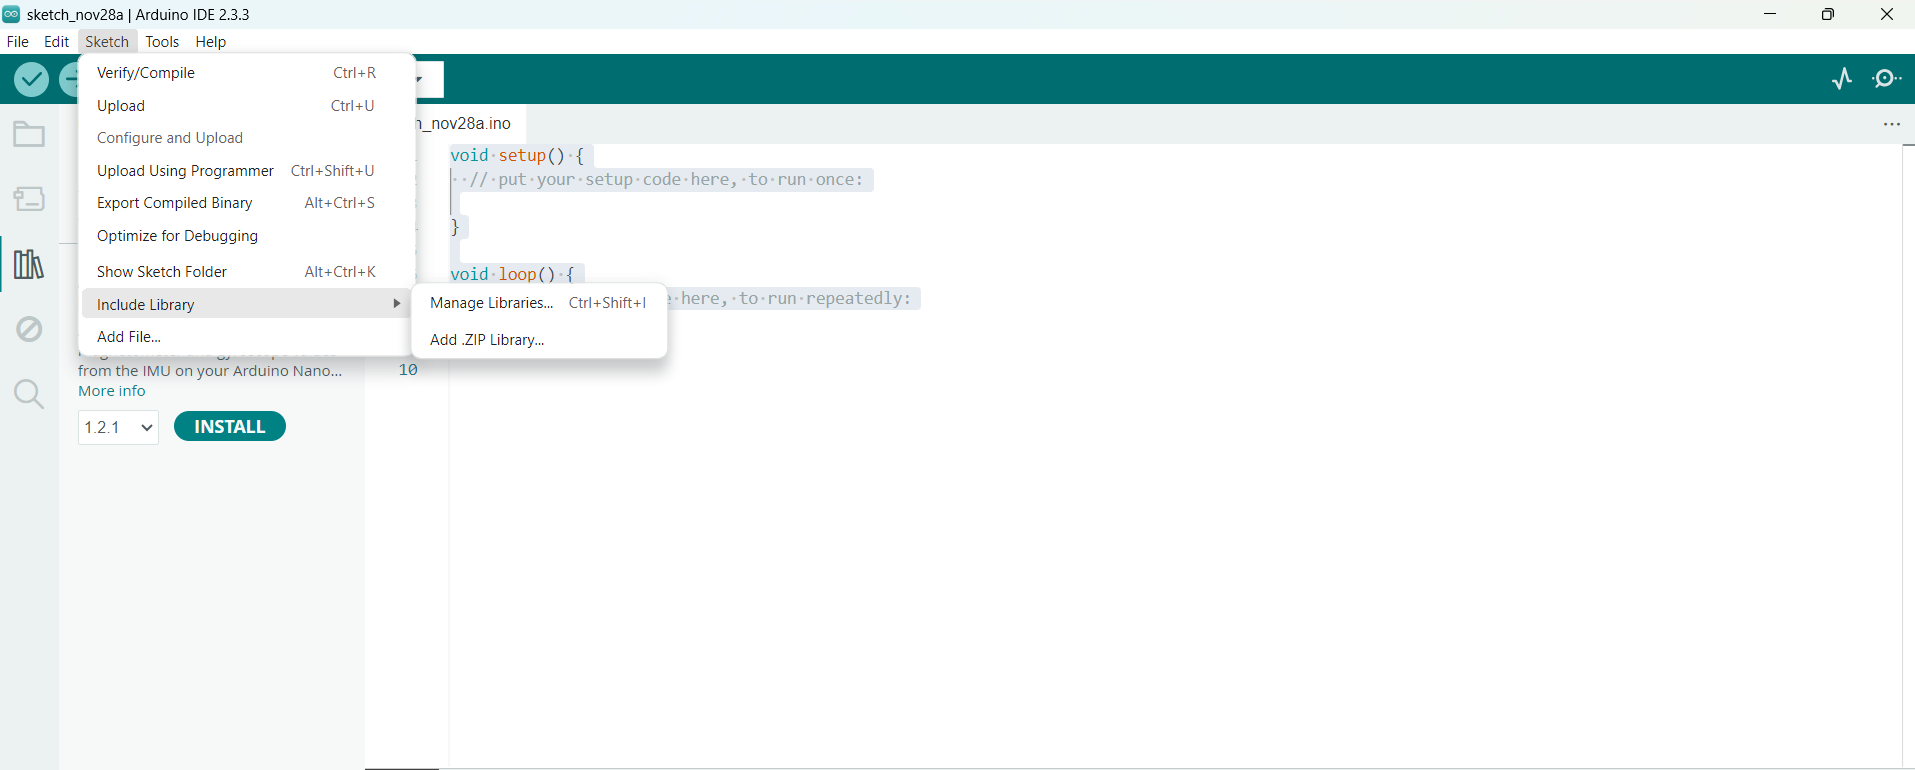
\includegraphics[width=0.7\textwidth]{Images/LibraryInstallingPath}
		\caption {Path for installing libraries.}
		\label{fig:librarypath}
	\end{figure}
	
	\subsection*{First Steps (GUI/UI Description)}
	The Arduino IDE provides several tools and buttons to help you write, compile, and upload code to your Arduino board. Below is a description of the essential GUI features:
	
	\begin{itemize}
		\item \textbf{Verify/Upload:}
		\begin{itemize}
			\item \textbf{Verify:} Checks your code for syntax errors without uploading it to the board. It's the first step to ensure your program is error-free.
			\item \textbf{Upload:} Sends your verified code to the connected Arduino board for execution.
		\end{itemize}
		
		\item \textbf{Select Board \& Port:}
		\begin{itemize}
			\item \textbf{Board Selection:} Specify the type of Arduino board you are using (e.g., Nano 33 BLE Sense) via the \texttt{Tools > Board} menu. This ensures compatibility with your code.
			\item \textbf{Port Selection:} Choose the port where your Arduino is connected (e.g., \texttt{COM3} on Windows or \texttt{/dev/ttyUSB0} on Linux). This allows the IDE to communicate with the board.
		\end{itemize}
		
		\item \textbf{Open Serial Monitor:} Displays real-time text output from the Arduino board. Useful for debugging and monitoring sensor readings or program output.
		
		\item \textbf{Open Serial Plotter:} Visualizes numerical data from the Arduino in a real-time graph. Ideal for monitoring sensor trends, such as accelerometer or gyroscope readings.
		
		\item \textbf{Search:} Quickly find and navigate code or settings within your sketch using the magnifying glass icon or \texttt{Ctrl+F} (Windows/Linux) or \texttt{Cmd+F} (macOS).
		
		\item \textbf{Debugger (Pro Feature):} Available in the Arduino IDE Pro version, it allows step-by-step code execution, variable inspection, and breakpoint setting for advanced debugging.
		
		\item \textbf{Library Manager:} Access via \texttt{Sketch > Include Library > Manage Libraries}. Lets you search for, install, and update libraries, like BMI270\_BMM150, to expand Arduino's functionality.
		
		\item \textbf{Board Manager:} Access via \texttt{Tools > Board > Board Manager}. Install or update support packages for different Arduino boards, including the Nano 33 BLE Sense Rev 2.
		
		\item \textbf{Sketchbook:} A repository of saved sketches (Arduino programs). Access it through the \texttt{File > Sketchbook} menu for easy management of your projects\cite{ArduinoIDE:2024}.
	\end{itemize}
	
\begin{figure}[h]
	\centering
	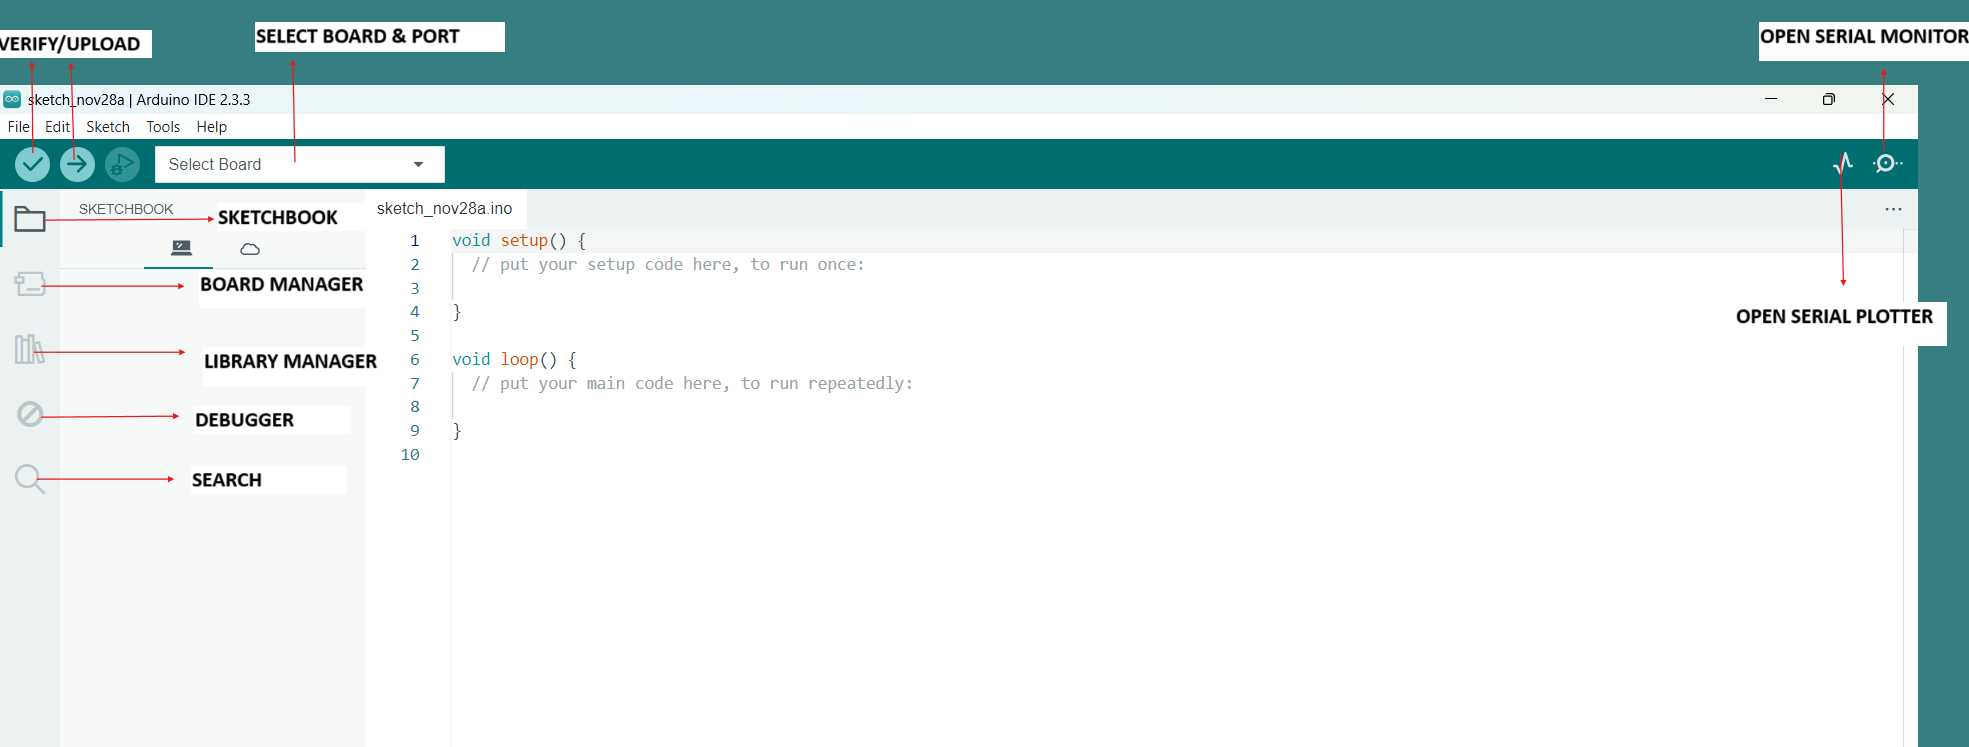
\includegraphics[width=0.7\textwidth]{Images/IDEBasicTools}
	\caption {Features of Arduino IDE.}
	\label{fig:IDE UI}
\end{figure}
	
	As shown in Figure\ref{fig:IDE UI}, the Arduino IDE interface includes essential features such as the code editor, the verify/upload buttons, and tools for selecting the board and port, making it easy to write and upload programs to the Arduino board.
	
	\subsubsection*{Arduino ``Hello World'' Program}
	\begin{lstlisting}[language=C++, caption=Simple Arduino Hello World Program]
		void setup() {
			Serial.begin(9600);  // Start communication with the computer
			while (!Serial);     // Wait for the Serial Monitor to open
			Serial.println("Hello, World!");  // Print "Hello, World!" to the Serial Monitor
		}
		
		void loop() {
			// Nothing here for a simple Hello World program
		}
	\end{lstlisting}
	
	To run:
	\begin{enumerate}
		\item Copy the code into the Arduino IDE.
		\item Click \textbf{Verify} (checkmark icon) to ensure the code has no errors.
		\item Click \textbf{Upload} (arrow icon) to send the program to the Arduino board.
		\item Open the \textbf{Serial Monitor} (magnifying glass icon) to see the output:
		\begin{lstlisting}
			Hello, World!
		\end{lstlisting}
	\end{enumerate}
	
	\subsubsection*{Linux Bash Script for Gait Recognition Data Collection}
	\begin{lstlisting}[language=bash, caption=Bash Script to Log Gait Data]
		#!/bin/bash
		
		# Script to log gait data from Arduino Serial output
		PORT="/dev/ttyUSB0"  # Replace with your Arduino's port
		BAUD="9600"
		LOGFILE="gait_data.log"
		
		echo "Starting data logging..."
		stty -F $PORT $BAUD
		cat $PORT > $LOGFILE
		echo "Data logged to $LOGFILE"
	\end{lstlisting}
	
	To run:
	\begin{enumerate}
		\item Save the script as \texttt{log\_gait\_data.sh}.
		\item Make it executable:
		\begin{lstlisting}[language=bash]
			chmod +x log_gait_data.sh
		\end{lstlisting}
		\item Run the script:
		\begin{lstlisting}[language=bash]
			./log_gait_data.sh
		\end{lstlisting}
		\item The collected data will be saved in \texttt{gait\_data.log}.
	\end{enumerate}
	